\documentclass[11pt,a4paper]{article}

\usepackage[utf8x]{inputenc}   % omogoča uporabo slovenskih črk kodiranih v formatu UTF-8
\usepackage[slovene]{babel}    % naloži, med drugim, slovenske delilne vzorce

\usepackage[hyphens]{url}
\usepackage{hyperref}

\usepackage{graphicx}

\usepackage{tikz}
\usetikzlibrary{arrows,calc,positioning,shadows,shapes}


\title{Akcijski načrt za mojo diplomsko nalogo:\\
``Perspektiva''}
\author{Aljoša Rakita\\
aljo.aljo.aljo@hotmail.com\\
\ \\
predvideni MENTOR: (doc./prof.) dr. Franc Solina \\
Fakulteta za računalništvo in informatiko Univerze v Ljubljani
\date{\today}         
}



\begin{document}
\maketitle

\section{Katere aktivnosti so potrebne za izdelavo moje diplomske naloge --- akcijski načrt}



\begin{itemize}
  \item ideja za diplomo (konkreten razmislek o temi diplome -> tema diplomskega dela) 1 mesec
  \item iskanje mentorja (sestanek v živo, pisanje emailov -> mentor diplomskega dela) 1 teden
  \item \v{s}tudij literature (iskanje, branje, pisanje povzetkov -> teoretična podlaga) 2 meseca
  \item pisanje dispozicije (pisanje -> dispozicija) 1 teden
  \item kodiranje (kodiranje, testiranje -> program) 1 mesec
  \item anketiranje (sestavljanje ankete, čakanje in analiza rezultatov -> delujoč program) 2 tedna
  \item pisanje diplome (razmišlanje, pisanje, preverjanje -> napisana diploma) 1 mesec
  \item zagovor(priprava na zagovor,zagovarjanje -> opravljena diploma) 1 mesec
\end{itemize}

\section{Kako so identificirane aktivnosti povezane med seboj}

Na sliki \ref{sl:mreza} je prikazan  diagram aktivnosti za diplomsko nalogo.

\begin{figure}[htb]
\resizebox{\textwidth}{!}{
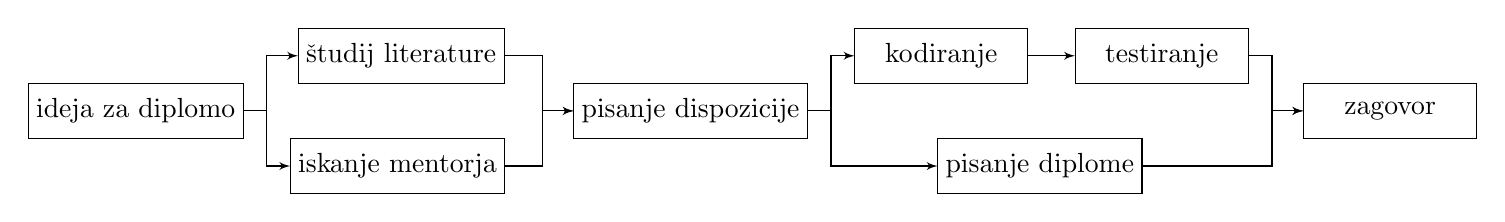
\begin{tikzpicture}[
            > = latex',
node distance = 0mm and 3mm,
mynode/.style = {name=n#1,
                 draw, minimum height=7mm, minimum width=22mm,
                 inner sep=1mm, outer sep = 0mm}
                        ]
%---
\node[mynode=1]                                                            {ideja za diplomo};
\node[mynode=2,above right=0mm and 7mm of n1]      {\v{s}tudij literature};
\node[mynode=3,right=42mm of n1]                               {pisanje dispozicije};
\node[mynode=4,above right=0mm and 6mm of n3]      {kodiranje};
\node[mynode=5,right=0mm and 6mm of n4]                 {testiranje};
\node[mynode=6,below right=0mm and 6mm of n1]       {iskanje mentorja};
\node[mynode=7,right=20mm and 55mm of n6]             {pisanje diplome};
\node[mynode=8, right=63mm of n3]                              {zagovor};
%---
\coordinate[right=3mm of n1]    (a);
\coordinate[left=4mm of n3]    (b);
\coordinate[right=3mm of n3.east]    (c);
\coordinate[left=4mm of n8.west]    (d);
%---
\draw       (n1) -- (a);
\draw[->]   (a) |- (n2);
\draw[->]   (a) |- (n6);
%
\draw[->]   (n6.east) -| (b) -- (b -| n3.west);
\draw[->]   (n2.east) -| (b) -- (b -| n3.west);
%
\draw  (n3.east) -- (c);
\draw[->]   (c) |- (n4.west);
\draw[->]   (c) |- (n7.west);
%
\draw[->]   (n4) -- (n5);
%
\draw[->]    (n5.east) -| (d) -- (d -| n8.west);
\draw[->]    (n7.east) -| (d) -- (d -| n8.west);

%-------
    \end{tikzpicture}
}
\caption{Mrežni diagram aktivnosti za diplomsko nalogo.}
\label{sl:mreza}
\end{figure}


\section{Časovna analiza in optimizacija načrta}

Ocene časa trajanja posameznih aktivnosti so navedene v prvi točki.
Le te se seštejejo  v sedem mesecev, kar mislim da je dokaj optimistično in primerno, zato menim, da časa trajanja ni potrebno krajšati.


\end{document}  




